Ainda que um extra, ou talvez mesmo não um extra uma vez que é uma componente de desenvolvimento não de jogo, criamos também um módulo para profiling. Existem três arrays para armazenar os valores:

\begin{description}
\item[\textit{start}] Regista o tempo no início da medição.
\item[\textit{end}] Regista o tempo no final da medição.
\item[\textit{name}] Regista a descrição da medição.
\end{description}

A utilização é intuitiva. É invocado o método start\_time com um identificador e uma descrição, ou nome no inicio da medição e end\_time com o mesmo identificador no final da medição. Invocado o render é impresso para o ecrã a subtração entre tempo final e inicial associado à descrição.

\begin{lstlisting}[caption=Métodos para trabalhar com profiling.]
void start_time(int num, char* name);
void end_time(int num);
void render();
\end{lstlisting}

\begin{figure}[here]
                 \centering{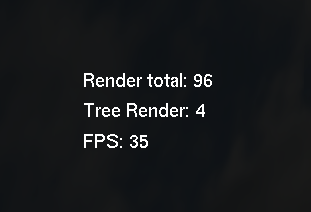
\includegraphics[width=0.3\textwidth]{images/prof.png}}
                 \caption{Profilling.}
                 \label{fig:prototype}
\end{figure}
